% generated by Plantuml 1.2025.7       
\definecolor{plantucolor0000}{RGB}{0,0,0}
\definecolor{plantucolor0001}{RGB}{225,245,254}
\definecolor{plantucolor0002}{RGB}{2,136,209}
\definecolor{plantucolor0003}{RGB}{1,87,155}
\definecolor{plantucolor0004}{RGB}{255,243,224}
\definecolor{plantucolor0005}{RGB}{230,81,0}
\definecolor{plantucolor0006}{RGB}{191,54,12}
\definecolor{plantucolor0007}{RGB}{243,229,245}
\definecolor{plantucolor0008}{RGB}{106,27,154}
\definecolor{plantucolor0009}{RGB}{74,20,140}
\definecolor{plantucolor0010}{RGB}{254,255,221}
\definecolor{plantucolor0011}{RGB}{24,24,24}
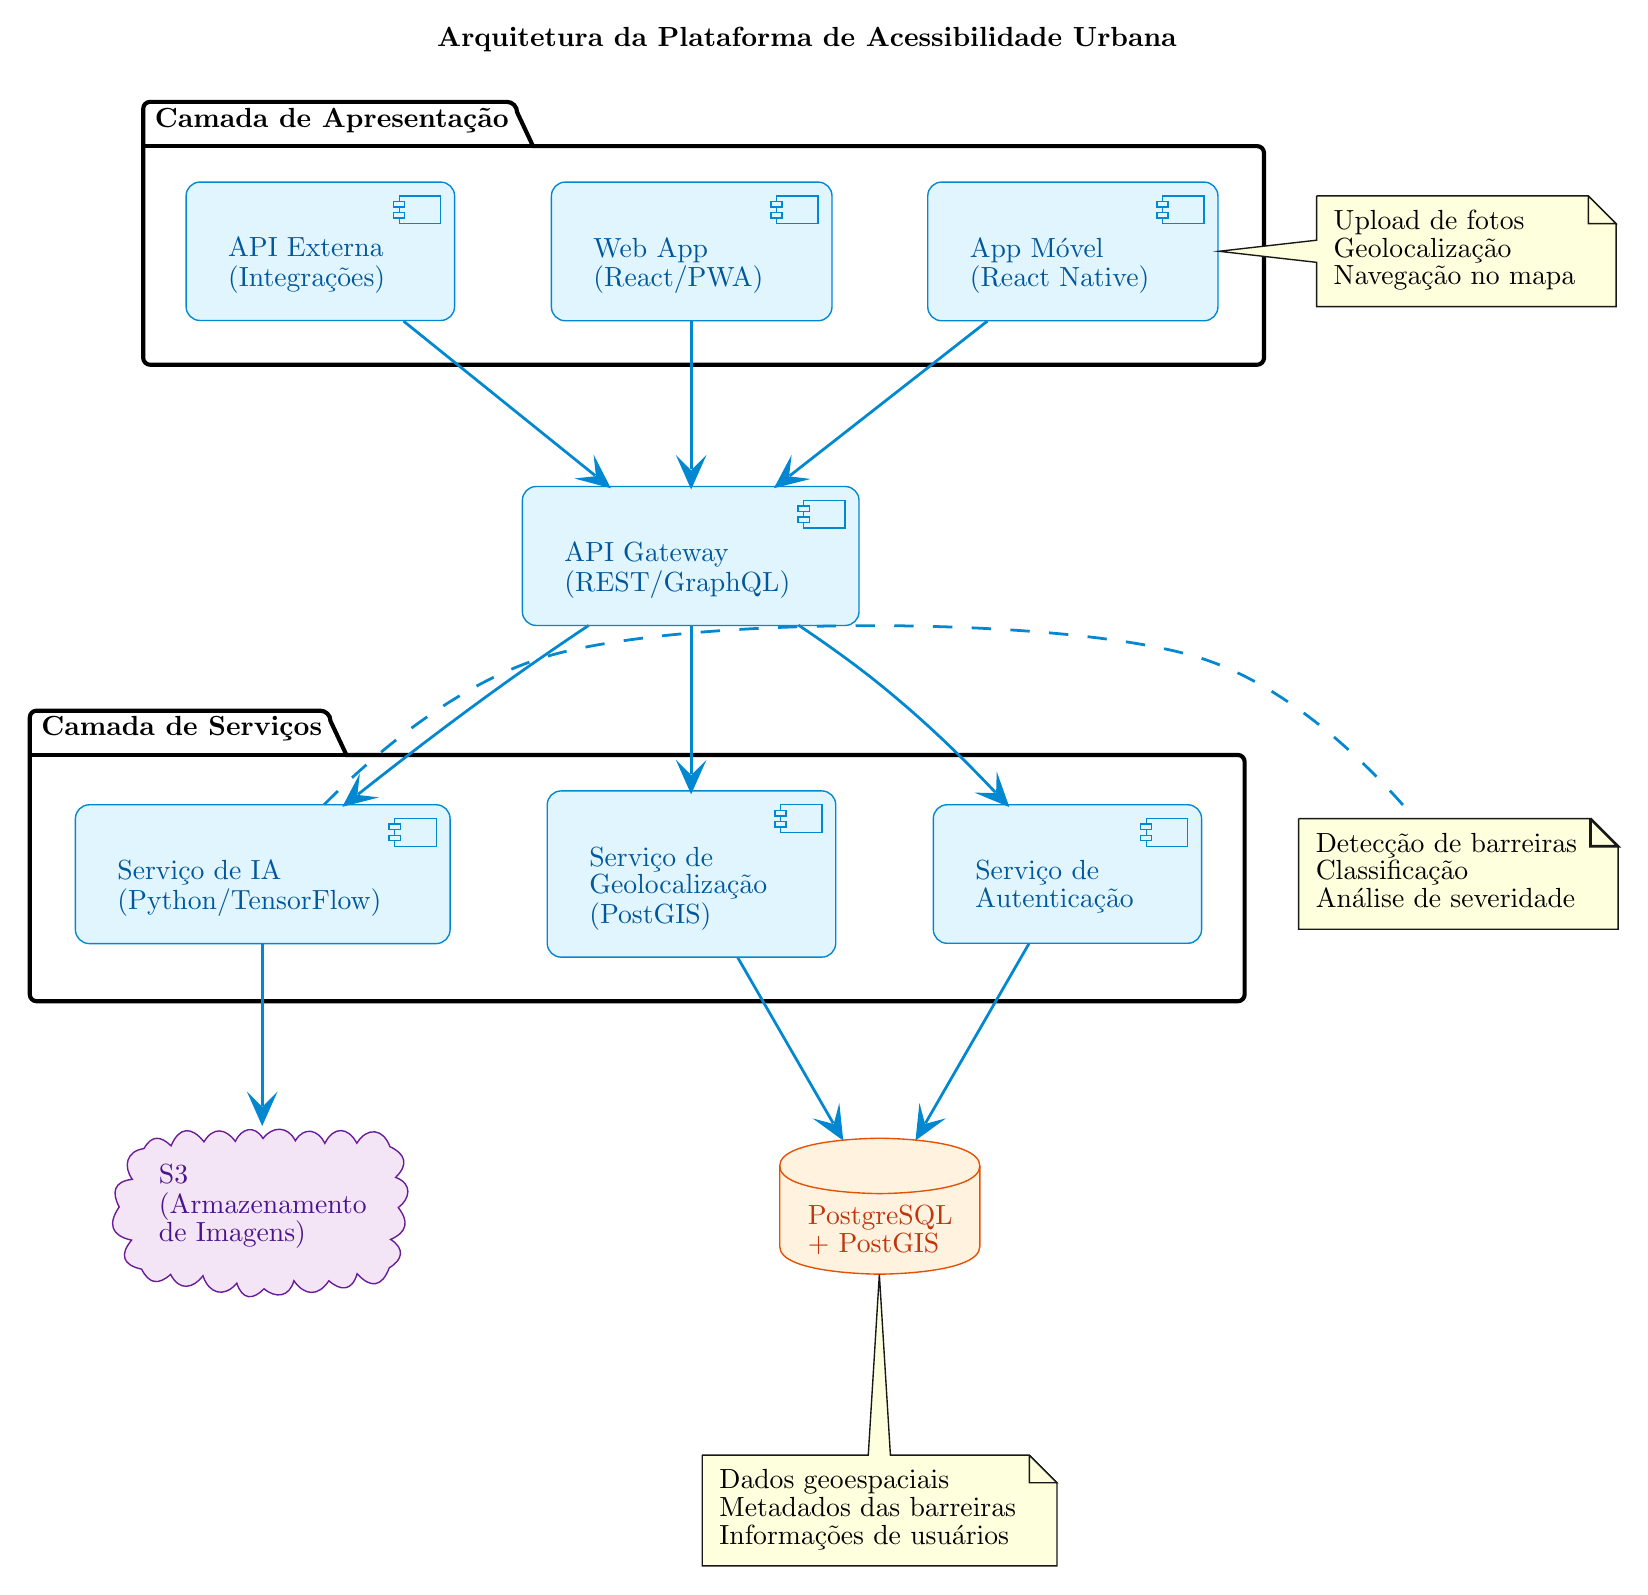
\begin{tikzpicture}[yscale=-1
,pstyle0/.style={color=black,line width=1.5pt}
,pstyle1/.style={color=plantucolor0002,fill=plantucolor0001,line width=0.5pt}
,pstyle5/.style={color=plantucolor0011,fill=plantucolor0010,line width=0.5pt}
,pstyle7/.style={color=plantucolor0002,line width=1.0pt}
,pstyle8/.style={color=plantucolor0002,fill=plantucolor0002,line width=1.0pt}
]
\node at (153.045pt,10pt)[below right,color=black,inner sep=0]{\textbf{Arquitetura da Plataforma de Acessibilidade Urbana}};
\draw[pstyle0] (49.5pt,37pt) -- (178.35pt,37pt) arc(270:360:3.75pt)  -- (187.85pt,53pt) -- (449.5pt,53pt) arc(270:360:2.5pt)  -- (452pt,129.5pt) arc(0:90:2.5pt)  -- (49.5pt,132pt) arc(90:180:2.5pt)  -- (47pt,39.5pt) arc(180:270:2.5pt) ;
\draw[pstyle0] (47pt,53pt) -- (187.85pt,53pt);
\node at (51pt,39pt)[below right,color=black,inner sep=0]{\textbf{Camada de Apresentação}};
\draw[pstyle0] (8.5pt,257pt) -- (110.93pt,257pt) arc(270:360:3.75pt)  -- (120.43pt,273pt) -- (442.5pt,273pt) arc(270:360:2.5pt)  -- (445pt,359.5pt) arc(0:90:2.5pt)  -- (8.5pt,362pt) arc(90:180:2.5pt)  -- (6pt,259.5pt) arc(180:270:2.5pt) ;
\draw[pstyle0] (6pt,273pt) -- (120.43pt,273pt);
\node at (10pt,259pt)[below right,color=black,inner sep=0]{\textbf{Camada de Serviços}};
\draw[pstyle1] (330.5pt,71pt) arc (180:270:5pt) -- (335.5pt,66pt) -- (430.35pt,66pt) arc (270:360:5pt) -- (435.35pt,71pt) -- (435.35pt,111.1pt) arc (0:90:5pt) -- (430.35pt,116.1pt) -- (335.5pt,116.1pt) arc (90:180:5pt) -- (330.5pt,111.1pt) -- cycle;
\draw[pstyle1] (415.35pt,71pt) rectangle (430.35pt,81pt);
\draw[pstyle1] (413.35pt,73pt) rectangle (417.35pt,75pt);
\draw[pstyle1] (413.35pt,77pt) rectangle (417.35pt,79pt);
\node at (345.5pt,86pt)[below right,color=plantucolor0003,inner sep=0]{App Móvel};
\node at (345.5pt,96.1pt)[below right,color=plantucolor0003,inner sep=0]{(React Native)};
\draw[pstyle1] (194.5pt,71pt) arc (180:270:5pt) -- (199.5pt,66pt) -- (290.89pt,66pt) arc (270:360:5pt) -- (295.89pt,71pt) -- (295.89pt,111.1pt) arc (0:90:5pt) -- (290.89pt,116.1pt) -- (199.5pt,116.1pt) arc (90:180:5pt) -- (194.5pt,111.1pt) -- cycle;
\draw[pstyle1] (275.89pt,71pt) rectangle (290.89pt,81pt);
\draw[pstyle1] (273.89pt,73pt) rectangle (277.89pt,75pt);
\draw[pstyle1] (273.89pt,77pt) rectangle (277.89pt,79pt);
\node at (209.5pt,86pt)[below right,color=plantucolor0003,inner sep=0]{Web App};
\node at (209.5pt,96.1pt)[below right,color=plantucolor0003,inner sep=0]{(React/PWA)};
\draw[pstyle1] (62.5pt,71pt) arc (180:270:5pt) -- (67.5pt,66pt) -- (154.52pt,66pt) arc (270:360:5pt) -- (159.52pt,71pt) -- (159.52pt,111pt) arc (0:90:5pt) -- (154.52pt,116pt) -- (67.5pt,116pt) arc (90:180:5pt) -- (62.5pt,111pt) -- cycle;
\draw[pstyle1] (139.52pt,71pt) rectangle (154.52pt,81pt);
\draw[pstyle1] (137.52pt,73pt) rectangle (141.52pt,75pt);
\draw[pstyle1] (137.52pt,77pt) rectangle (141.52pt,79pt);
\node at (77.5pt,86pt)[below right,color=plantucolor0003,inner sep=0]{API Externa};
\node at (77.5pt,96pt)[below right,color=plantucolor0003,inner sep=0]{(Integrações)};
\draw[pstyle1] (22.5pt,296pt) arc (180:270:5pt) -- (27.5pt,291pt) -- (152.88pt,291pt) arc (270:360:5pt) -- (157.88pt,296pt) -- (157.88pt,336.16pt) arc (0:90:5pt) -- (152.88pt,341.16pt) -- (27.5pt,341.16pt) arc (90:180:5pt) -- (22.5pt,336.16pt) -- cycle;
\draw[pstyle1] (137.88pt,296pt) rectangle (152.88pt,306pt);
\draw[pstyle1] (135.88pt,298pt) rectangle (139.88pt,300pt);
\draw[pstyle1] (135.88pt,302pt) rectangle (139.88pt,304pt);
\node at (37.5pt,311pt)[below right,color=plantucolor0003,inner sep=0]{Serviço de IA};
\node at (37.5pt,321.16pt)[below right,color=plantucolor0003,inner sep=0]{(Python/TensorFlow)};
\draw[pstyle1] (193pt,291pt) arc (180:270:5pt) -- (198pt,286pt) -- (292.23pt,286pt) arc (270:360:5pt) -- (297.23pt,291pt) -- (297.23pt,341.05pt) arc (0:90:5pt) -- (292.23pt,346.05pt) -- (198pt,346.05pt) arc (90:180:5pt) -- (193pt,341.05pt) -- cycle;
\draw[pstyle1] (277.23pt,291pt) rectangle (292.23pt,301pt);
\draw[pstyle1] (275.23pt,293pt) rectangle (279.23pt,295pt);
\draw[pstyle1] (275.23pt,297pt) rectangle (279.23pt,299pt);
\node at (208pt,306pt)[below right,color=plantucolor0003,inner sep=0]{Serviço de};
\node at (208pt,316.05pt)[below right,color=plantucolor0003,inner sep=0]{Geolocalização};
\node at (208pt,326.05pt)[below right,color=plantucolor0003,inner sep=0]{(PostGIS)};
\draw[pstyle1] (332.5pt,296pt) arc (180:270:5pt) -- (337.5pt,291pt) -- (424.44pt,291pt) arc (270:360:5pt) -- (429.44pt,296pt) -- (429.44pt,336.05pt) arc (0:90:5pt) -- (424.44pt,341.05pt) -- (337.5pt,341.05pt) arc (90:180:5pt) -- (332.5pt,336.05pt) -- cycle;
\draw[pstyle1] (409.44pt,296pt) rectangle (424.44pt,306pt);
\draw[pstyle1] (407.44pt,298pt) rectangle (411.44pt,300pt);
\draw[pstyle1] (407.44pt,302pt) rectangle (411.44pt,304pt);
\node at (347.5pt,311pt)[below right,color=plantucolor0003,inner sep=0]{Serviço de};
\node at (347.5pt,321.05pt)[below right,color=plantucolor0003,inner sep=0]{Autenticação};
\draw[pstyle1] (184pt,181pt) arc (180:270:5pt) -- (189pt,176pt) -- (300.65pt,176pt) arc (270:360:5pt) -- (305.65pt,181pt) -- (305.65pt,221.21pt) arc (0:90:5pt) -- (300.65pt,226.21pt) -- (189pt,226.21pt) arc (90:180:5pt) -- (184pt,221.21pt) -- cycle;
\draw[pstyle1] (285.65pt,181pt) rectangle (300.65pt,191pt);
\draw[pstyle1] (283.65pt,183pt) rectangle (287.65pt,185pt);
\draw[pstyle1] (283.65pt,187pt) rectangle (287.65pt,189pt);
\node at (199pt,196pt)[below right,color=plantucolor0003,inner sep=0]{API Gateway};
\node at (199pt,206.21pt)[below right,color=plantucolor0003,inner sep=0]{(REST/GraphQL)};
\draw[color=plantucolor0005,fill=plantucolor0004,line width=0.5pt] (277pt,421.5pt) ..controls (277pt,411.5pt) and (313.155pt,411.5pt) .. (313.155pt,411.5pt) ..controls (313.155pt,411.5pt) and (349.31pt,411.5pt) .. (349.31pt,421.5pt) -- (349.31pt,450.61pt) ..controls (349.31pt,460.61pt) and (313.155pt,460.61pt) .. (313.155pt,460.61pt) ..controls (313.155pt,460.61pt) and (277pt,460.61pt) .. (277pt,450.61pt) -- (277pt,421.5pt);
\draw[color=plantucolor0005,line width=0.5pt] (277pt,421.5pt) ..controls (277pt,431.5pt) and (313.155pt,431.5pt) .. (313.155pt,431.5pt) ..controls (313.155pt,431.5pt) and (349.31pt,431.5pt) .. (349.31pt,421.5pt);
\node at (287pt,435.5pt)[below right,color=plantucolor0006,inner sep=0]{PostgreSQL};
\node at (287pt,445.61pt)[below right,color=plantucolor0006,inner sep=0]{+ PostGIS};
\draw[color=plantucolor0008,fill=plantucolor0007,line width=0.5pt] (47.2552pt,415.2421pt) ..controls (50.1329pt,410.2453pt) and (53.3106pt,410.6453pt) .. (57.0669pt,414.2385pt) ..controls (60.0163pt,407.2572pt) and (64.4747pt,407.1497pt) .. (68.96pt,412.7915pt) ..controls (72.3333pt,407.233pt) and (76.7668pt,407.9012pt) .. (80.2833pt,412.6338pt) ..controls (82.4092pt,408.0174pt) and (87.1322pt,406.4179pt) .. (90.2813pt,411.5884pt) ..controls (93.6841pt,407.0263pt) and (99.2712pt,406.9965pt) .. (101.9777pt,412.4053pt) ..controls (105.1459pt,407.0275pt) and (110.3735pt,408.453pt) .. (112.6341pt,413.3468pt) ..controls (115.76pt,407.1091pt) and (121.0068pt,407.2638pt) .. (124.185pt,413.2976pt) ..controls (127.924pt,407.2814pt) and (133.7384pt,407.9182pt) .. (136.1569pt,414.5477pt) ..controls (141.8222pt,417.2087pt) and (142.9762pt,421.0605pt) .. (138.2035pt,425.6462pt) ..controls (144.4206pt,427.9022pt) and (143.4852pt,433.3846pt) .. (139.1616pt,436.5655pt) ..controls (143.1071pt,441.5689pt) and (142.3984pt,445.4526pt) .. (136.3956pt,448.0626pt) ..controls (141.6437pt,451.4099pt) and (140.7628pt,455.4328pt) .. (135.9161pt,458.3076pt) ..controls (133.2808pt,465.3166pt) and (129.2336pt,465.8597pt) .. (124.2975pt,460.4622pt) ..controls (122.46pt,466.762pt) and (118.4413pt,466.7904pt) .. (114.0891pt,463.0084pt) ..controls (110.2159pt,468.7877pt) and (105.3067pt,468.4673pt) .. (101.4467pt,462.9936pt) ..controls (99.7667pt,469.0017pt) and (94.872pt,469.4106pt) .. (90.6404pt,465.8859pt) ..controls (86.6134pt,470.1532pt) and (82.7587pt,469.8246pt) .. (80.8215pt,463.877pt) ..controls (76.1538pt,469.4077pt) and (70.6456pt,467.529pt) .. (68.6034pt,461.1773pt) ..controls (65.1035pt,465.8442pt) and (59.9765pt,466.8528pt) .. (56.9206pt,460.6979pt) ..controls (52.4913pt,464.638pt) and (49.1525pt,464.1716pt) .. (46.4064pt,458.7979pt) ..controls (39.6712pt,457.3576pt) and (38.3526pt,453.6115pt) .. (42.7994pt,448.3214pt) ..controls (35.2587pt,446.6779pt) and (34.2073pt,442.3107pt) .. (38.3322pt,436.3236pt) ..controls (35.508pt,431.0365pt) and (36.363pt,427.0867pt) .. (43.082pt,426.3397pt) ..controls (39.7019pt,421.8041pt) and (40.88pt,416.1093pt) .. (47.2552pt,415.2421pt);
\node at (52.5pt,421pt)[below right,color=plantucolor0009,inner sep=0]{S3};
\node at (52.5pt,431pt)[below right,color=plantucolor0009,inner sep=0]{(Armazenamento};
\node at (52.5pt,441pt)[below right,color=plantucolor0009,inner sep=0]{de Imagens)};
\draw[pstyle5] (471pt,71pt) -- (471pt,87pt) -- (435.7pt,91pt) -- (471pt,95pt) -- (471pt,111pt) -- (471pt,111pt) -- (579.21pt,111pt) -- (579.21pt,111pt) -- (579.21pt,81pt) -- (569.21pt,71pt) -- (471pt,71pt) -- (471pt,71pt);
\draw[pstyle5] (569.21pt,71pt) -- (569.21pt,81pt) -- (579.21pt,81pt) -- (569.21pt,71pt);
\node at (477pt,76pt)[below right,color=black,inner sep=0]{Upload de fotos};
\node at (477pt,86pt)[below right,color=black,inner sep=0]{Geolocalização};
\node at (477pt,96pt)[below right,color=black,inner sep=0]{Navegação no mapa};
\draw[pstyle5] (464.5pt,296pt) -- (464.5pt,336pt) -- (579.93pt,336pt) -- (579.93pt,306pt) -- (569.93pt,296pt) -- (464.5pt,296pt);
\draw[color=plantucolor0011,fill=plantucolor0010,line width=1.0pt] (569.93pt,296pt) -- (569.93pt,306pt) -- (579.93pt,306pt) -- (569.93pt,296pt);
\node at (470.5pt,301pt)[below right,color=black,inner sep=0]{Detecção de barreiras};
\node at (470.5pt,311pt)[below right,color=black,inner sep=0]{Classificação};
\node at (470.5pt,321pt)[below right,color=black,inner sep=0]{Análise de severidade};
\draw[pstyle5] (249pt,526pt) -- (249pt,566pt) -- (249pt,566pt) -- (377.2pt,566pt) -- (377.2pt,566pt) -- (377.2pt,536pt) -- (367.2pt,526pt) -- (317pt,526pt) -- (313pt,460.7pt) -- (309pt,526pt) -- (249pt,526pt) -- (249pt,526pt);
\draw[pstyle5] (367.2pt,526pt) -- (367.2pt,536pt) -- (377.2pt,536pt) -- (367.2pt,526pt);
\node at (255pt,531pt)[below right,color=black,inner sep=0]{Dados geoespaciais};
\node at (255pt,541pt)[below right,color=black,inner sep=0]{Metadados das barreiras};
\node at (255pt,551pt)[below right,color=black,inner sep=0]{Informações de usuários};
\draw[pstyle7] (352.03pt,116.24pt) ..controls (329.3pt,134.02pt) and (303.2956pt,154.3828pt) .. (280.5956pt,172.1428pt);
\draw[pstyle8] (275.87pt,175.84pt) -- (285.4231pt,173.4446pt) -- (279.808pt,172.759pt) -- (280.4936pt,167.1439pt) -- (275.87pt,175.84pt) -- cycle;
\draw[pstyle7] (245pt,116.24pt) ..controls (245pt,134.02pt) and (245pt,152.08pt) .. (245pt,169.84pt);
\draw[pstyle8] (245pt,175.84pt) -- (249pt,166.84pt) -- (245pt,170.84pt) -- (241pt,166.84pt) -- (245pt,175.84pt) -- cycle;
\draw[pstyle7] (141.07pt,116.24pt) ..controls (163.14pt,134.02pt) and (188.3072pt,154.3163pt) .. (210.3572pt,172.0763pt);
\draw[pstyle8] (215.03pt,175.84pt) -- (210.5299pt,167.0793pt) -- (211.136pt,172.7036pt) -- (205.5117pt,173.3097pt) -- (215.03pt,175.84pt) -- cycle;
\draw[pstyle7] (207.98pt,226.17pt) ..controls (197.24pt,233.36pt) and (185.56pt,241.37pt) .. (175pt,249pt) ..controls (156.37pt,262.46pt) and (140.7248pt,274.4965pt) .. (124.6148pt,287.2465pt);
\draw[pstyle8] (119.91pt,290.97pt) -- (129.4496pt,288.5212pt) -- (123.8307pt,287.867pt) -- (124.4848pt,282.2481pt) -- (119.91pt,290.97pt) -- cycle;
\draw[pstyle7] (245pt,226.24pt) ..controls (245pt,243.75pt) and (245pt,261.48pt) .. (245pt,279.99pt);
\draw[pstyle8] (245pt,285.99pt) -- (249pt,276.99pt) -- (245pt,280.99pt) -- (241pt,276.99pt) -- (245pt,285.99pt) -- cycle;
\draw[pstyle7] (283.75pt,226.07pt) ..controls (294.19pt,233.07pt) and (305.28pt,241pt) .. (315pt,249pt) ..controls (330.64pt,261.87pt) and (342.6206pt,273.5471pt) .. (355.0006pt,286.5971pt);
\draw[pstyle8] (359.13pt,290.95pt) -- (355.8378pt,281.6677pt) -- (355.6888pt,287.3226pt) -- (350.0339pt,287.1736pt) -- (359.13pt,290.95pt) -- cycle;
\draw[pstyle7] (261.81pt,346.17pt) ..controls (273.37pt,366.23pt) and (285.5323pt,387.3525pt) .. (296.3523pt,406.1125pt);
\draw[pstyle8] (299.35pt,411.31pt) -- (298.3184pt,401.5153pt) -- (296.8519pt,406.9788pt) -- (291.3885pt,405.5122pt) -- (299.35pt,411.31pt) -- cycle;
\draw[pstyle7] (90pt,341.16pt) ..controls (90pt,359.91pt) and (90pt,379.96pt) .. (90pt,399.86pt);
\draw[pstyle8] (90pt,405.86pt) -- (94pt,396.86pt) -- (90pt,400.86pt) -- (86pt,396.86pt) -- (90pt,405.86pt) -- cycle;
\draw[pstyle7] (367.08pt,341.16pt) ..controls (355.26pt,361.66pt) and (341.4061pt,385.7016pt) .. (329.6661pt,406.0716pt);
\draw[pstyle8] (326.67pt,411.27pt) -- (334.6297pt,405.4697pt) -- (329.1667pt,406.938pt) -- (327.6985pt,401.475pt) -- (326.67pt,411.27pt) -- cycle;
\draw[color=plantucolor0002,line width=1.0pt,dash pattern=on 7.0pt off 7.0pt] (112.37pt,290.95pt) ..controls (131.43pt,271.76pt) and (160.72pt,247.01pt) .. (192.5pt,237.5pt) ..controls (242.53pt,222.53pt) and (377.47pt,222.53pt) .. (427.5pt,237.5pt) ..controls (460.4pt,247.34pt) and (489.29pt,275.85pt) .. (506.21pt,295.66pt);
\end{tikzpicture}
